\documentclass[conference]{IEEEtran}
\IEEEoverridecommandlockouts

\usepackage{cite}
\usepackage{amsmath,amssymb,amsfonts}
\usepackage{algorithm}
\usepackage{algpseudocode}
\usepackage{graphicx}
\usepackage{textcomp}
\usepackage{xcolor}
\usepackage{booktabs}
\usepackage{hyperref}
\usepackage{pgfplots}
\usepackage{array}
\usepackage{makecell}
\pgfplotsset{compat=1.18}

% ✅ Add this just before \begin{document}
\linespread{0.96}

\def\BibTeX{{\rm B\kern-.05em{\sc i\kern-.025em b}\kern-.08em
    T\kern-.1667em\lower.7ex\hbox{E}\kern-.125emX}}

\title{Strings Attached: A Performance Analysis of Levenshtein and Hamming Distance \\
Comparative Study for String Matching Applications}



\author{\IEEEauthorblockN {Vishakha Joshi}
\IEEEauthorblockA{\textit{Department of Computer Engg} \\
\textit{NMIMS, Navi Mumbai}\\
Mumbai, Maharashtra \\
vishakha.joshi515@gmail.com}
\and
\IEEEauthorblockN {Devshree Marathe}
\IEEEauthorblockA{\textit{Department of Computer Engg} \\
\textit{NMIMS, Navi Mumbai}\\
Mumbai, Maharashtra \\
devshreemarathe@gmail.com}
\and
\IEEEauthorblockN{Ashmit Kotiya}
\IEEEauthorblockA{\textit{Department of Computer Engg} \\
\textit{NMIMS, Navi Mumbai}\\
Mumbai, Maharashtra \\
kotiyaashmit@gmail.com}
}



\begin{document}
\maketitle

\begin{abstract}
String matching is a basic computer science problem and finds applications in numerous areas including text processing, bioinformatics, and spell-checking. String matching aims at establishing the similarity between two strings, which is vital for applications such as autocorrect, DNA sequence alignment, and data retrieval. String matching may be either exact (when two strings should exactly match) or approximate (when small variations are tolerated) based on the problem.
This paper contrasts two basic approximate string matching algorithms
\begin{enumerate}
    \item Levenshtein Distance (Edit Distance) – Quantifies the minimum number of insertions, deletions, and substitutions to change one string into another.
    \item Hamming Distance – Enumerates the number of differing characters between two strings but with the condition that they have the same length.
\end{enumerate}
\end{abstract}

\begin{IEEEkeywords}
Levenshtein Distance, Hamming Distance, String Matching, Edit Distance, Approximate Algorithms, Performance Comparison
\end{IEEEkeywords}

\section{Introduction}
String matching is a core problem in information technology, and is one of the most prevalent issues in the computational complexity theory of algorithms. It is used widely in the fields of text editing processing, image processing, document retrieval, natural language recognition and biological sciences, etc. Besides, string matching is the most important time-consuming question of those applications. Improved string matching algorithms can considerably profit their application efficiencies. Research and design of a quick string search algorithm has strong theoretical and practical relevance.[7]

The two algorithms are very common but have different applications. Levenshtein Distance is more used in case of word comparisons of varying lengths, for instance, spell-checking and natural language processing, where one has to detect and correct slight typos. Hamming Distance, being more effective with fixed-length strings, finds applications in data transmission error detection and DNA sequence comparison.

The primary trade-off between such algorithms is efficiency vs. accuracy. Levenshtein Distance offers a more general and accurate similarity measure, but at the cost of increased time complexity of O(mn) (where m and n represent string lengths). Hamming Distance, on the other hand, is quicker with O(n) complexity, but without support for insertions and deletions, restricting its applicability to applications involving variable string lengths.

By this comparative analysis, we elucidate the advantage and limitation of each approach and offer an explanation of when and why to use each according to speed, accuracy, and computational efficiency.

\section{Approximate String Matching Algorithms}

\subsection{Levenshtein Distance}
The Levenshtein distance (LD) algorithm calculates the distance between two distinct phonetic sequences by identifying their discrepancies. The three primary steps of the Levenshtein distance algorithm are substitutions, deletions, and insertions [8]. Two phonetic segments can be aligned using the Levenshtein distance. It constructs a 2D table where each cell D[i][j]D[i][j] represents the minimum edit distance between the first ii characters of one string and the first jj characters of the other, with the final cell D[m][n]D[m][n] providing the total edit distance.

The Levenshtein Distance Algorithm is extensively employed to find the similarity of two strings in terms of the minimum edits—insertions, deletions, or substitutions—to convert one string into another. It is applied in a vast range of applications from spell checking and auto-correct, where it provides a close enough word for misspelled words, to plagiarism detection by finding similarities in texts and DNA sequence analysis to detect mutations or evolutionary divergences. The algorithm is utilized through speech and optical character recognition (OCR) through voice-to-text and correction of scanned documents, improves search engines and fuzzy matching by improving search results on misspellings, and enables natural language processing (NLP) to detect variations in words in text processing. As a computationally efficient means of detecting differences between strings, it is a fundamental tool in a range of applications involving text comparison and similarity measurement.

\begin{algorithm}
\caption{Levenshtein Distance between \texttt{str1} and \texttt{str2}}
\begin{algorithmic}[1]
\State $m \gets \text{length of } \texttt{str1}$
\State $n \gets \text{length of } \texttt{str2}$
\State Create a matrix $dp$ of size $(m+1) \times (n+1)$
\For{$i \gets 0$ to $m$}
    \State $dp[i][0] \gets i$
\EndFor
\For{$j \gets 0$ to $n$}
    \State $dp[0][j] \gets j$
\EndFor
\For{$i \gets 1$ to $m$}
    \For{$j \gets 1$ to $n$}
        \If{$\texttt{str1}[i-1] = \texttt{str2}[j-1]$}
            \State $cost \gets 0$
        \Else
            \State $cost \gets 1$
        \EndIf
        \State $dp[i][j] \gets \min\Big\{
      \begin{aligned}
      &dp[i{-}1][j] + 1, \\
      &dp[i][j{-}1] + 1, \\
      &dp[i{-}1][j{-}1] + cost
      \end{aligned}
      \Big\}$  
    \EndFor
\EndFor
\State \Return $dp[m][n]$
\end{algorithmic}
\end{algorithm}

\textbf{Strengths:} The Levenshtein Distance Algorithm is strong across many domains that make it widely applicable. It is intuitive and easy to understand because the process of counting deletions, substitutions, and insertions is easy to comprehend and apply. It is flexible due to which it is suitable to be used across many applications including spell checking, NLP, DNA sequence comparison, and plagiarism. The algorithm is efficient in handling words of different lengths and hence is ideal to be used in comparing strings of different lengths. It also detects major differences by measuring the "effort" required to convert one string to another due to which it is an ideal tool to use in measuring similarity. It is also ideal to be used across short strings, handling short text inputs like names, words, and short sentences.

\textbf{Weaknesses:} The Levenshtein Distance Algorithm suffers some disadvantages that make it inefficient and not practical to use. It is computationally expensive, with time complexity of (O(m*n)), and thus slow to calculate for long strings. It is context-insensitive, i.e., it assigns equal weight to all edits, when in actuality some transformations (e.g., substituting "ph" with "f") are more common in actual use. The algorithm is also phonetically blind, i.e., two homophones spelled the same, e.g., "knight" and "nite," can have high distance. It also uses a lot of memory since it requires a 2D table of size (m*n), which is memory-intensive for long strings. Lastly, it is limited to exact edits and does not allow transpositions, e.g., exchanging two adjacent characters (e.g., "hte" → "the").


\subsection{Hamming Distance}
Hamming distance is a measure to compare two strings (or vectors) of the same length. It is a measure of the number of positions where the corresponding symbols differ. Introduced first by Richard Hamming in error-detecting and error-correcting codes, this metric is now of central importance in a wide range of fields including coding theory, information theory, and bioinformatics.

The Hamming distance is widely applied in the following ways:
\begin{enumerate}
    \item Error Detection/Correction: In coding theory, it is used to determine how many errors have occurred during the transmission of a code word.
    \item Data Clustering and Classification: It is used as a measure of similarity in different machine learning algorithms.
    \item Bioinformatics: For comparison of genetic sequences, where each nucleotide is encoded as a character.
\end{enumerate}

The most straightforward algorithm to compute the Hamming distance between two sequences involves a single pass through both sequences, comparing the corresponding elements. If the elements differ, a counter is incremented. The final value of the counter represents the Hamming distance.
\begin{algorithm}
\caption{Hamming Distance between A and B}
\begin{algorithmic}[1]  % ✅ Add [1] here to enable numbering
\Require Two sequences $A$ and $B$
\Ensure The Hamming distance between $A$ and $B$
\If{Length($A$) $\neq$ Length($B$)}
    \State \textbf{raise error} "Sequences must be of equal length"
\EndIf
\State $distance \gets 0$
\For{$i \gets 0$ to Length($A$)$ - 1$}
    \If{$A[i] \neq B[i]$}
        \State $distance \gets distance + 1$
    \EndIf
\EndFor
\State \Return $distance$
\end{algorithmic}
\end{algorithm}

\textbf{Strengths:} The Hamming Distance algorithm is appreciated for its simpleness, since it only keeps track of the number of positions where two strings of the same length differ. Its efficiency is impressive, in linear time O(n), where n represents the number of characters in the strings, and it only uses constant additional space. It also fulfills the formal requirements of a metric non-negativity, identity, symmetry, and the triangle inequality—so it is appropriate for theoretical and practical uses. The algorithm finds special utility in certain fields like error detection and correction in coding theory, particularly where binary or fixed-length information is found, such as in digital communication systems. Additionally, its algorithmic simplicity allows it to be relatively easily implemented in a wide range of programming languages and platforms.

\textbf{Weaknesses:} The Hamming Distance algorithm has a number of limitations that impact its usability in more complicated situations. Its equal-length requirement makes it only suitable for comparing strings or sequences of equal length, making it less useful in situations where inputs vary in size. It is also not sensitive to the type of substitutions, considering all mismatches as equal without regard to the extent or importance of the difference between symbols. This equal weighting might be unsuitable in applications where some substitutions have greater significance than others. Further, the algorithm cannot process insertions or deletions, so it isn't as well-suited for sequence comparison applications where these types of operations are frequent—situations where more adaptable measures such as Levenshtein Distance are more suitable. Its binary over-simplification also makes it less effective in subtle fields such as natural language processing or bioinformatics, wherein it is important to capture fine similarities. Finally, Hamming Distance is sensitive to misalignments; even a small misalignment of sequences can result in a large distance value, though the content itself is actually very similar.

\section{Result and Discussion}

\subsection{Performance Analysis on Strings of Similar Pattern}
A thorough performance analysis of the Levenshtein Distance as well as Hamming Distance algorithms is imperative with respect to the criteria of "similar patterns" under which such tiny changes in the two strings would be best recognized by either algorithm concerned. Both the algorithms, under consideration, are exceptional with respect to similar strings, while both are different in one respect. The flexibility and robustness of Levenshtein Distance about near matches are with insertions, deletions, and substitutions as compared to Hamming. If "SPARE", and "SHIRE" are provided as inputs, this fact leads to Levenshtein distance value as 2 - replacement of one 'P' by 'H,' and similarly, another 'A' is replaced by 'I.' As a result, the similarity degree in the two cases strongly exceeds either of the characters' positions. And thus the Hamming Distance would apply only in the case where the two strings compared were of equal lengths and then only measure the actual number of mismatches between characters found at corresponding positions. Hamming Distance would in this situation return 2 because 'P' and 'A' differ from 'H' and 'I' in their respective positions. However, in this case, even though both return an equivalent numerical value, Levenshtein, in customary sense, is more powerful with reference to finding similar patterns because it can deal with strings of different lengths using different types of edits and thus affords it a much better circumstance on programmatic fuzzy matching, which Hamming does not allow at all without a corresponding position misplacing.


\subsection{Performance Analysis on Strings of Varying Pattern}
The unequal performance levels are accentuated by analyzing the performance of Levenshtein Distance and Hamming Distance algorithms with respect to "different pattern." The actual cases would demonstrate that, because of Levenshtein Distance dealing with huge levels of deviations on structural changes among strings by incorporating insertions, deletions, and replacements, it works well for strings that have the most different patterns, such as using it on 'MATHEUS' and 'VIABLES' where the Levenshtein Distance of 6 says that it takes six operations of edit to transform one string into the other, replacing most of the characters and retaining just one or two (like 'S') in the process. That high distance signals how different they are, and Levenshtein measures it right. In these two strings' case, the Hamming Distance comes into play as the two strings are the same length (7) and count the mismatches 6 where only the last matching character is 'S.' This other one gives the same number mathematically, but poor semantically; otherwise, it calculates mismatch only in positions. For structurally different string pairs, the Levenshtein furthers its cause, counting the number of actual edits needed regardless of position, and thus is far more robust along other patterns.

\begin{figure}[htbp]
\centering
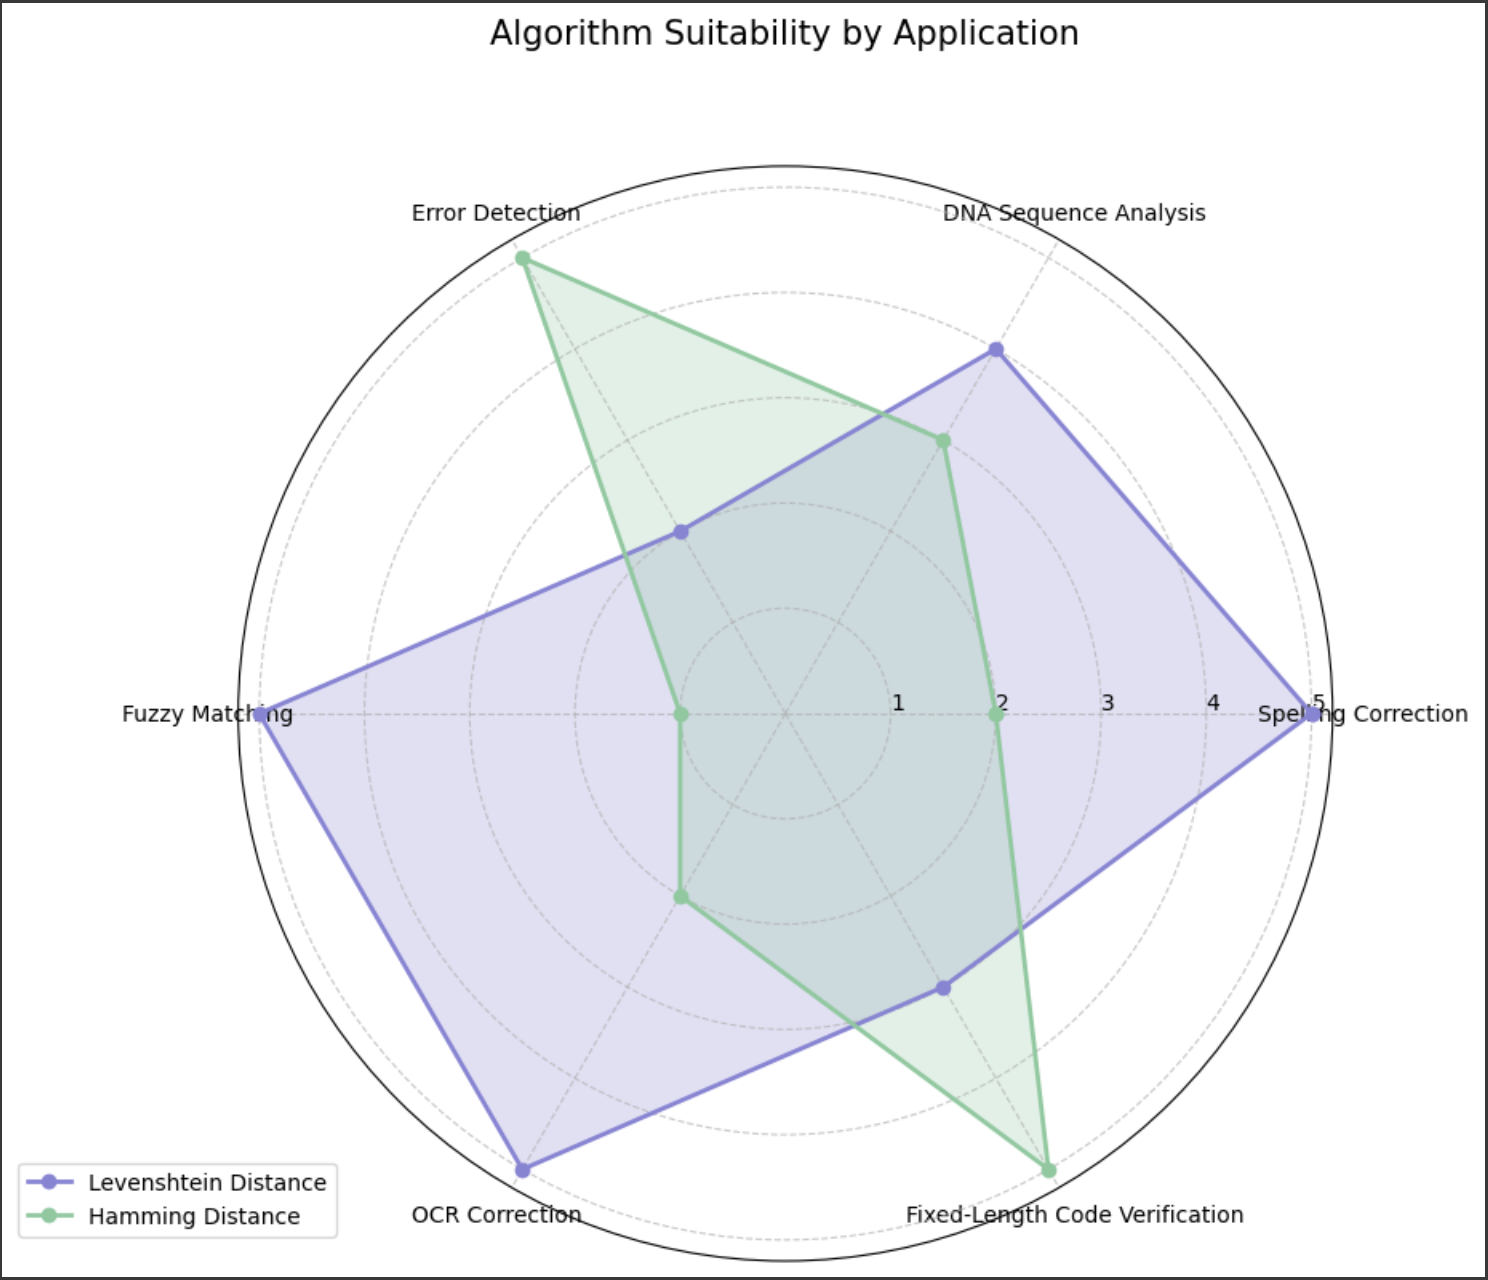
\includegraphics[width=0.48\textwidth]{application_suitability.png}
\caption{Algorithm suitability based on real-world applications. Levenshtein Distance performs better in fuzzy text applications (e.g., OCR, spelling correction), while Hamming Distance is more optimal for fixed-length use cases like error detection.}
\label{fig:application-suitability}
\end{figure}

\subsection{Complexity Analysis}
\begin{itemize}
\item Levenshtein: Time = $O(mn)$, Space = $O(mn)$
\item Hamming: Time = $O(n)$, Space = $O(1)$
\end{itemize}

\begin{table}[htbp]
\caption{Execution Time Comparison of String Matching Algorithms}
\centering
\renewcommand{\arraystretch}{1.2} % increases row height slightly
\begin{tabular}{|p{2.5cm}|p{2.6cm}|p{2.6cm}|}
\hline
\textbf{Input Strings} & \textbf{Algorithm Name} & \textbf{Execution Time} \\
\hline
Goldfish \& Waterway & Levenshtein Distance & 0.1080036163 \\
\hline
Goldfish \& Waterway & Hamming Distance & 0.0071525574 \\
\hline
Star \& Tsar & Levenshtein Distance & 0.0290870667 \\
\hline
Star \& Tsar & Hamming Distance & 0.0071525574 \\
\hline
Kitten \& Sitting & Levenshtein Distance & 0.0314712524 \\
\hline
Drought \& Crimson & Levenshtein Distance & 0.0305175781 \\
\hline
Drought \& Crimson & Hamming Distance & 0.0021457672 \\
\hline
\end{tabular}
\label{tab:execution_times}
\end{table}

\subsection{Comparison Metrics}
\begin{table}[htbp]
\caption{Comparison of Time and Space Complexity for String Matching Algorithms}
\centering
\scriptsize
\renewcommand{\arraystretch}{1.15}
\begin{tabular}{|p{2.2cm}|p{1.2cm}|p{1.5cm}|p{0.9cm}|}
\hline
\textbf{Algorithm} & \textbf{Time} & \textbf{Space} & \textbf{Stability} \\
\hline
Levenshtein Distance & $O(mn)$ & $O(mn)$ & Stable \\
\hline
\makecell[l]{Hamming \\ ($O(n)$ input)} & $O(n)$ & $O(1)$ & Stable \\
\hline
\end{tabular}
\label{tab:complexity}
\end{table}

\begin{figure}[htbp]
\centering
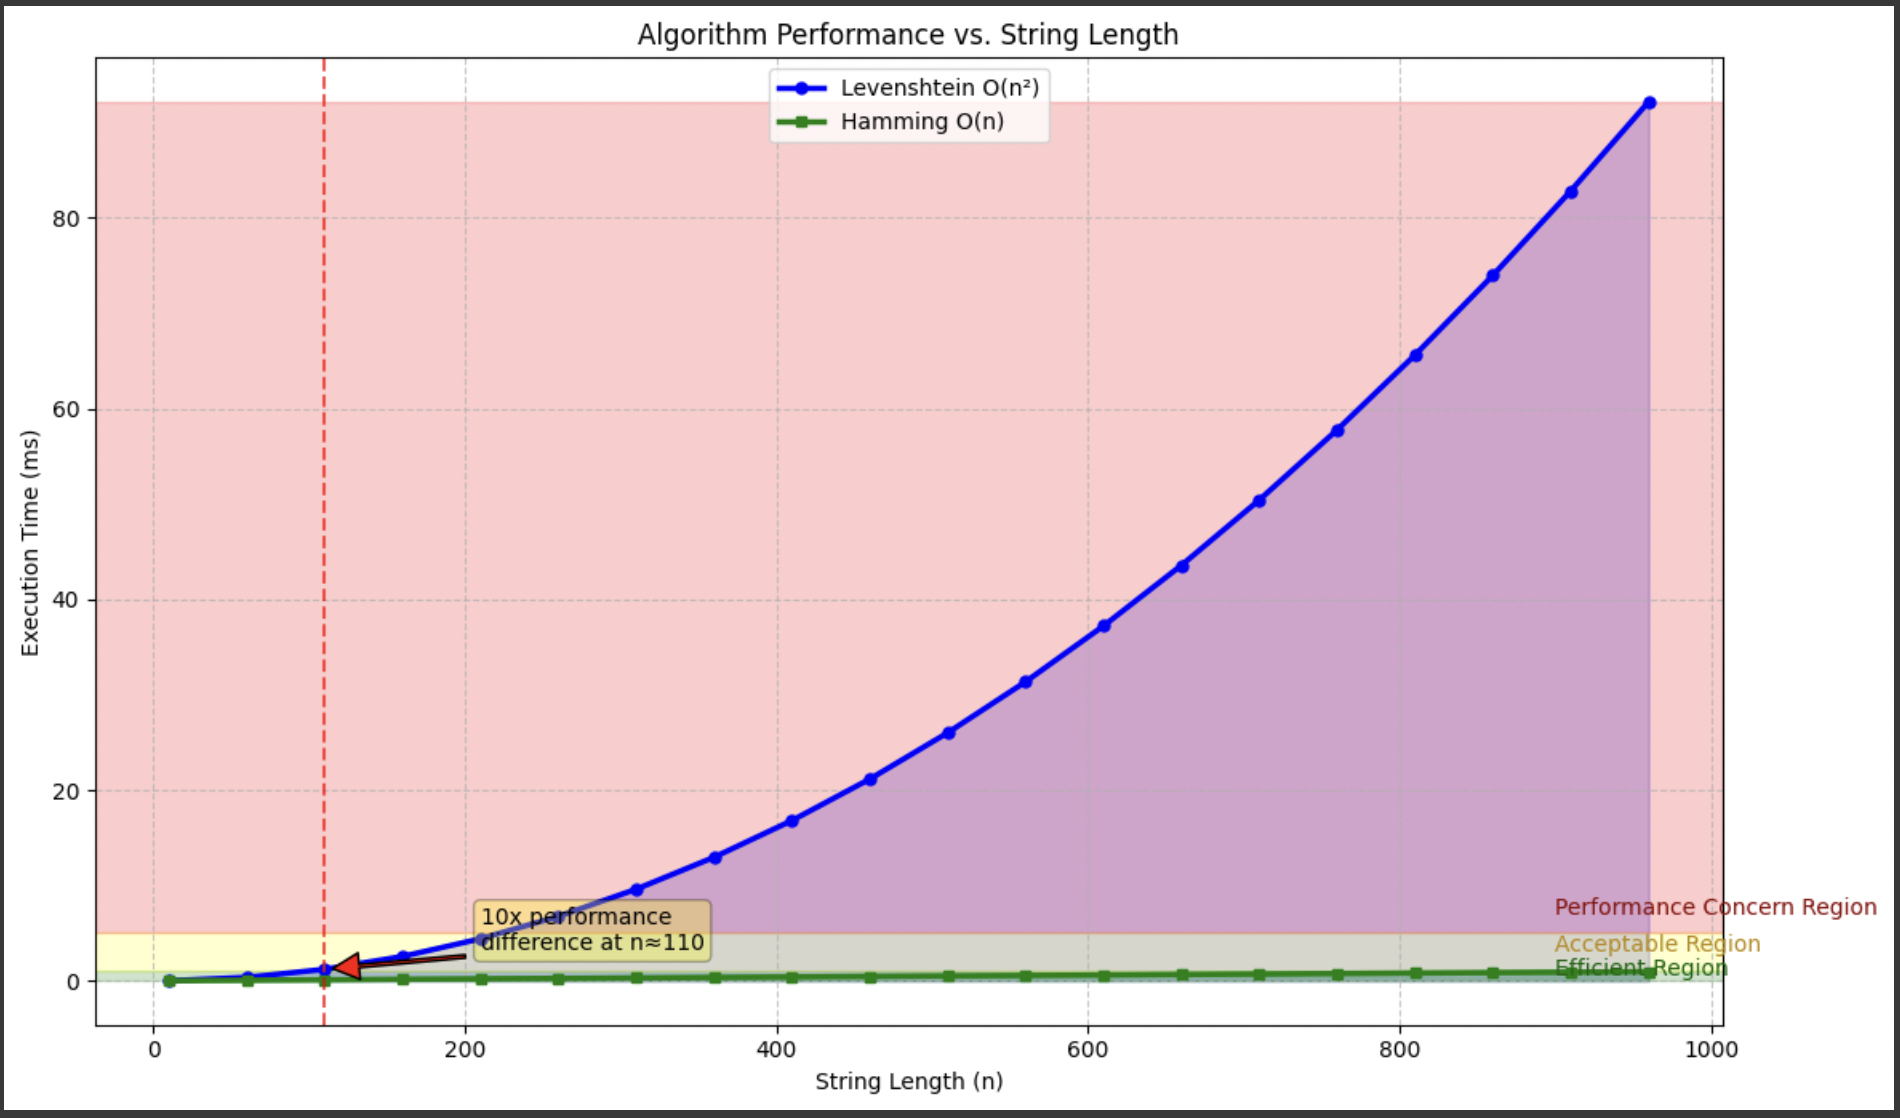
\includegraphics[width=0.48\textwidth]{performance_graph.png}
\caption{Algorithm performance comparison based on string length. Levenshtein Distance shows quadratic growth $O(n^2)$ while Hamming Distance grows linearly $O(n)$. The efficiency threshold is highlighted at $n \approx 110$, where a 10× performance gap is observed.}
\label{fig:performance-comparison}
\end{figure}

\begin{figure}[htbp]
\centering
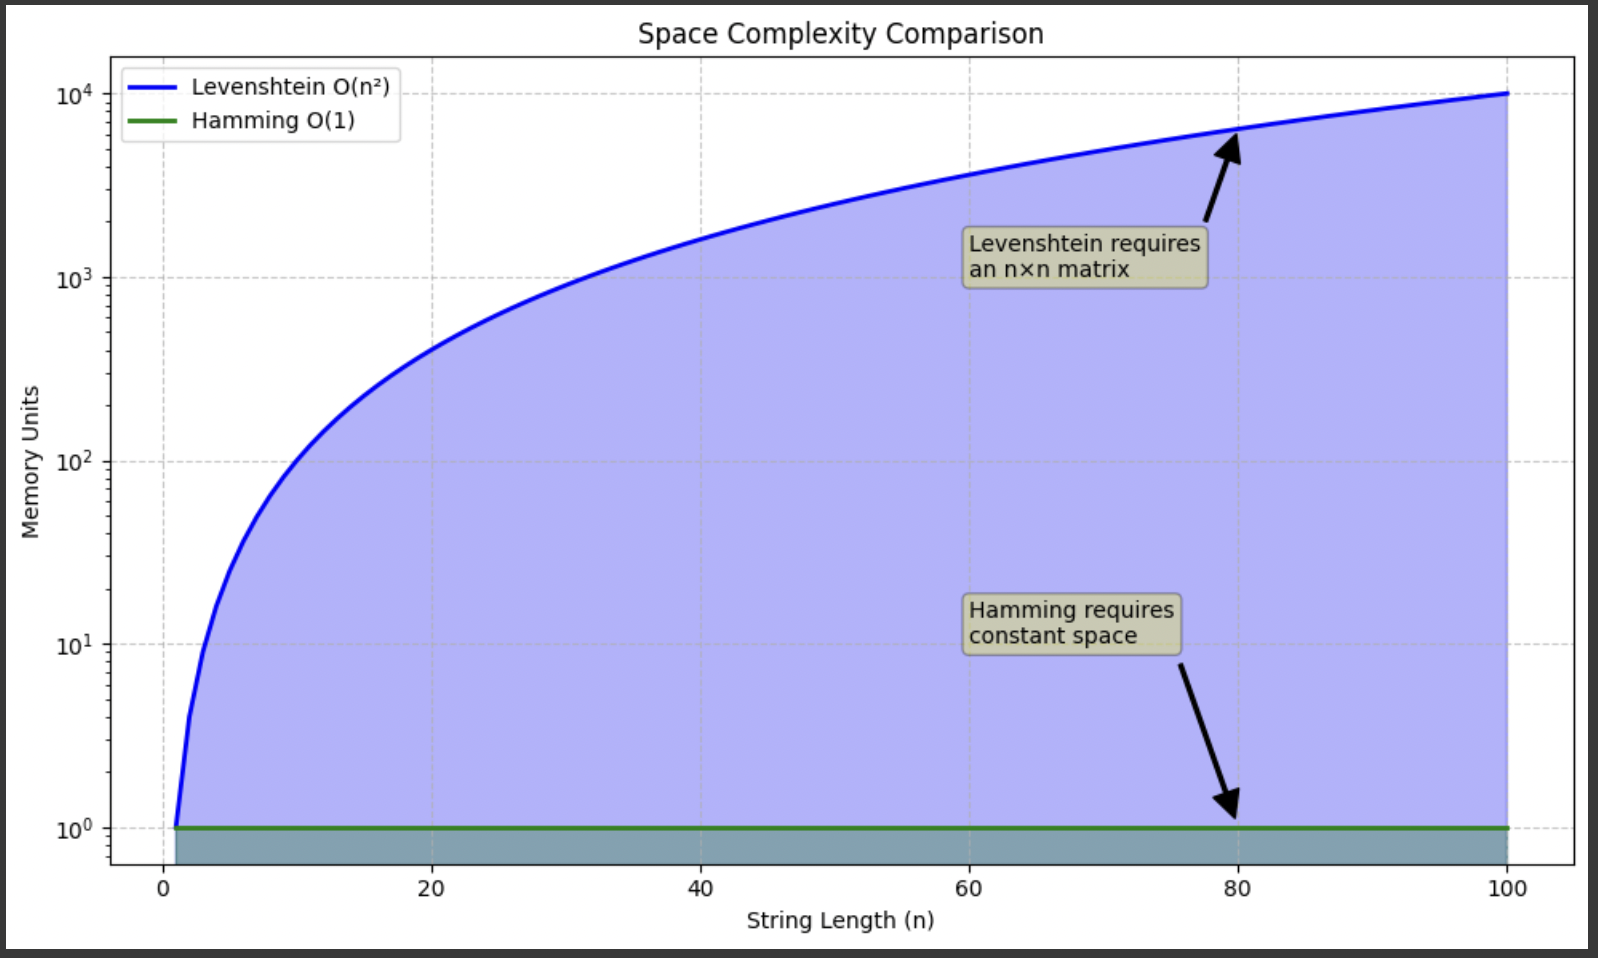
\includegraphics[width=0.48\textwidth]{space_complexity.png}
\caption{Space complexity comparison of string matching algorithms. Levenshtein Distance requires $O(n^2)$ space due to dynamic programming table, while Hamming Distance maintains $O(1)$ constant memory.}
\label{fig:space-comparison}
\end{figure}


The Levenshtein Distance, by using the dynamic programming approach, calculates the minimum number of editing operations such as insertions, deletions, or substitutions required to replace one string into another and usually fills in a matrix of size (m+1) × (n+1), where 'm' and 'n' represent the lengths of the two strings. Each cell then indicates the edit distance to be developed between prefixes in the strings. Therefore, the time complexity and space complexity both are O(m × n) due to the nested iteration over both strings and the storage of intermediate results in the 2D table, while Hamming Distance means only counting the positions at which two strings of equal length differ. Rather, it requires a single linear pass through the strings to calculate an O(n) time complexity and O(1) space complexity with a constant number of variables recognized for the input size. Hence, Hamming is considerably faster and lighter in weight than Levenshtein because it is better flexible than being suited for approximate string matching application, while Hamming is more suited for fixed lengths in string substitution.

\begin{table}[htbp]
\caption{Comparison of Additional Properties of String Matching Algorithms}
\centering
\scriptsize
\renewcommand{\arraystretch}{1.3}
\begin{tabular}{|p{2.2cm}|p{1.8cm}|p{2cm}|p{1.6cm}|}
\hline
\textbf{Algorithm} & \textbf{Recursion} & \textbf{Parallelisability} & \textbf{Robustness} \\
\hline
Levenshtein Distance & Possible (usually iterative) & Moderate (row/col-wise) & High — supports all edits \\
\hline
Hamming Distance & Not recursive & High (char-wise comparison) & Low — only substitutions \\
\hline
\multicolumn{4}{|c|}{\textbf{Implementation and Applications}} \\
\hline
\textbf{Algorithm} & \multicolumn{3}{p{5.4cm}|}{\centering \textbf{Implementation} and \textbf{Application}} \\
\hline
Levenshtein Distance & \multicolumn{3}{p{5.4cm}|}{
Requires 2D DP matrix; more memory-intensive. Used in spell checking, DNA alignment, OCR correction, NLP.
} \\
\hline
Hamming Distance & \multicolumn{3}{p{5.4cm}|}{
Simple loop; very light. Used in error detection, networking, and fixed-length comparisons.
} \\
\hline
\end{tabular}
\label{tab:str}
\end{table}



\section{Conclusion and Future Direction}
The comparison of Levenshtein Distance vs Hamming Distance highlights that both have individual strengths and limitations that are suited for specific uses. Hamming Distance is simple, highly efficient, and appropriate for matching strings of fixed size, particularly in areas of application like error detection, digital communications, and coding theory. But its effectiveness is compromised when applied to sequences of different lengths, insertions, deletions, or slight modifications—unqualified for sophisticated real-world data like natural language or biomolecular sequences. Levenshtein Distance is more flexible and robust, capable of identifying insertions, deletions, and substitutions, and superior for use like spell checking, DNA sequence alignment, and fuzzy string searching. It provides a more useful similarity score, but at the cost of increased computational resources.

Directions in the years to come could include the optimization of Levenshtein Distance for large-scale or real-time use with space-saving or parallelized algorithms. Hybrid approaches balancing the speed of Hamming Distance with the versatility of Levenshtein could also be explored for applications requiring performance and precision. Additionally, adapting these algorithms to incorporate weighted substitution or contextual resemblance (such as in semantic matching or NLP) can potentially render them more applicable to more advanced and intelligent systems. As pattern recognition and machine learning problems become increasingly challenging, merging data-driven models with distance metrics can potentially yield more adjustable and domain-based similarity measures.


\begin{thebibliography}{00}
\bibitem{b1} A Comparative Analysis of single pattern matching algorithms in text mining.
\bibitem{b2} String Matching Methodologies: A Comparative Analysis.
\bibitem{b3} Comparative study for better result on query suggestion of article searching with MySQL pattern matching and Jaccard similarity.
\bibitem{b4} String Matching Algorithms For Retrieving Information From Desktop – Comparative Analysis.
\bibitem{b5} New Hashing-Based Multiple String Pattern Matching Algorithms.
\bibitem{b6} Complexity Algorithm Analysis for Edit Distance.
\bibitem{b7} Comparison of two-dimensional string matching algorithms.
\end{thebibliography}


\end{document}